\documentclass[12pt]{article}

\usepackage[italian]{babel}
\usepackage[T1]{fontenc}
\usepackage{charter}
\usepackage{geometry}
\usepackage{graphicx}
\usepackage{float}
\usepackage{extsizes}
\usepackage{blindtext}
\usepackage{wrapfig}
\usepackage{ragged2e}
\usepackage{xcolor}
\usepackage{subcaption}
\usepackage{keyval}
\usepackage[format=plain, textfont=sl, font=footnotesize]{caption}
\usepackage{hyperref}

\geometry{
 a4paper,
 total={170mm,262mm},
 left=20mm,
 top=20mm,
 }
\graphicspath{ {res/} }
\hypersetup{
    colorlinks = false,
    pdftitle = {Smart Room Report},
    pdfpagemode=FullScreen,
}
\captionsetup[figure]{labelformat=empty, justification=centering}
\captionsetup[subfigure]{labelformat=empty, justification=centering}
\setlength\intextsep{0pt}
\def\code#1{\texttt{#1}}

\title{Smart Room}
\author{Marco Antolini, Luca Pasini, Lorenzo Tosi, Andrea Zavatta}

\begin{document}

\topskip0pt
\begin{center}
    \vspace*{\fill}
    \Huge\textbf{Relazione progetto Smart Room - IoT} \\
    \vspace*{\fill}
    \Large\textsl{Marco Antolini, Luca Pasini, Lorenzo Tosi, Andrea Zavatta} \\
    \vskip 1cm
    \large\textsl{marco.antolini6@studio.unibo.it, luca.pasini9@studio.unibo.it, lorenzo.tosi10@studio.unibo.it, andrea.zavatta3@studio.unibo.it}
    \vspace*{\fill}
\end{center}

\newpage

\tableofcontents
\newpage

% -------------------- Requisiti --------------------

\section{Requisiti}

Desideriamo realizzare un sistema IoT che implementi una versione semplificata di una stanza intelligente, finalizzata a monitorare e controllare lo stato di una stanza in un campus. \newline
1. Room Sensor Board (esp): Sistema incorporato per monitorare lo stato della stanza tramite sensori. Interagisce con il Room Service tramite MQTT o HTTP. \newline
2. Room Service (backend - pc): Funziona come unità principale per la gestione della stanza. Comunica tramite seriale con il Controller, tramite MQTT con la Room Sensor Board e tramite HTTP con la Dashboard. \newline
3. Room Controller (Arduino): Sistema incorporato che controlla la luce e le tapparelle. Comunica tramite seriale con il Room Service e tramite Bluetooth con la Room App. Deve implementare la logica di controllo tramite macchine a stati finiti (sincrone o asincrone). \newline
4. Room App (Android - smartphone): App mobile per il controllo manuale delle luci e delle tapparelle. Comunica con il Controller tramite Bluetooth (o tramite seriale in caso di emulatore Android). \newline
5. Room Dashboard (Frontend/web app su PC o tramite sockets): Interfaccia per visualizzare e tracciare lo stato della stanza. Interagisce con il Room Service. \newline
Il sistema Smart Room controlla l'illuminazione e le tapparelle secondo la seguente politica: \newline
- Se nessuno è nella stanza, la luce è spenta. \newline
- Se qualcuno entra in una stanza buia, la luce si accende. \newline
- Le tapparelle si sollevano completamente automaticamente alla prima entrata a partire dalle 8:00. \newline
- Le tapparelle si abbassano completamente alle 19:00 se sono sollevate e nessuno è in stanza, o non appena chi è ancora in stanza alle 19:00 lascia. \newline
Attraverso l'app mobile, l'utente può: \newline
- Accendere/spegnere la luce. \newline
- Sollevare/abbassare le tapparelle in modo parziale (0-100%). \newline
- Attraverso la dashboard, il responsabile della stanza può: \newline
- Monitorare lo stato della stanza. \newline
- Controllare completamente la luce e le tapparelle. \newline
- Si presume che la stanza sia accessibile dalle 8:00 alle 19:00. \newline
Ulteriori dettagli: \newline
- La Room Sensor Board deve accendere il LED quando qualcuno è in stanza e spegnerlo quando nessuno è presente. \newline
- Il Controller controlla/simula le tapparelle con un servomotore. 0° rappresenta le tapparelle completamente sollevate, 180° completamente abbassate.
\vskip 0.3cm
\begin{figure}[H]
    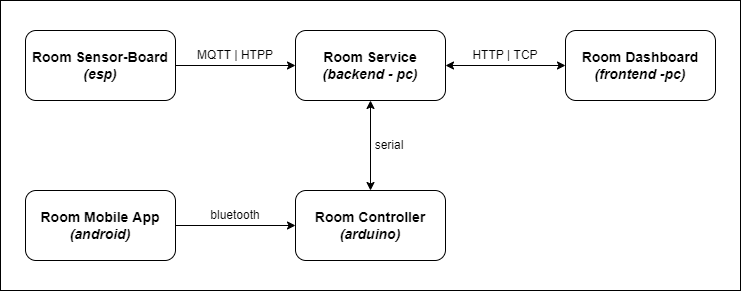
\includegraphics[width=17cm]{application-schema.png}
    \centering
    \caption{Schema funzionamento applicazione}
    \centering
\end{figure}

\newpage
% -------------------- Room Controller --------------------

\section{Room Controller}



\newpage
% -------------------- Room Sensor Board --------------------

\section{Room Sensor Board}



\newpage
% -------------------- Room Service --------------------

\section{Room Service}



\newpage
% -------------------- Room Dashboard --------------------

\section{Room Dashboard}

La Room Dashboard è un'applicazione web hostata su localhost grazie al servizio di web server Xampp che comunica tramite richieste HTTP con il Room Service per interagire con i componenti hardware.

\subsection{Interfaccia}

La dashboard comprende due pagine:
\newline
- Window: mostra lo stato attuale delle tapparelle e della lampadina all'interno della stanza e permette anche di modificarli;
\newline
- History: mostra dati relativi all'attività delle tapparelle e della lampadina.

\subsubsection{Window}
Nella Window è visibile un orologio che mostra l'orario attuale e lo sfondo del sito cambia dinamicamente in base al fatto che sia giorno o notte. È presente l'immagine di una lampadina che rispecchia lo stato della lampadina nella stanza e che è possibile cliccare per accendere e spegnere la luce. Accade lo stesso per le tapparelle, per cui è presente uno slider tramite il quale è possibile controllare l'apertura totale o parziale delle tapparelle della stanza.

\subsubsection{History}
Nella History sono presenti due logs che mostrano i momenti (con gli orari riportati in formato HH:mm:SS) in cui la lampadina è stata spenta o accesa (quindi rispettivamente con le diciture On o Off) e in cui la tapparella è stata aperta o chiusa (riportando la percentuale di apertura rilevata alla fine del movimento). \newline
Inoltre è presente un grafico a torta che mostra l'utilizzo della lampadina con due fette che raffigurano il tempo in cui è stata accesa e il tempo in cui è stata spenta e le relative percentuali. \newline
Tutti i dati riportati in questa pagina sono relativi alle ultime 24 ore.

\subsection{Software}
Come introdotto in precedenza la dashboard utilizza le richieste HTTP per comunicare con il Room Service in python che permette di scambiare informazioni e comandi in tempo reale con l'hardware. \newline
Tutti i logs delle ultime 24 ore vengono salvati (e aggiornati dinamicamente) sul file \code{logs.json}. \newline
Il file \code{room-dashboard-history.js} deve semplicemente accedere ai logs quindi fa una richiesta di tipo \code{GET} al file json ogni volta che la pagina viene aggiornata. \newline
Il file \code{room-dashboard-window.js} deve invece sia fare una richiesta di tipo \code{GET} al file json per ottenere i dati aggiornati, sia gestire i comandi provenienti dalla dashboard e farli arrivare all'hardware. Ciò avviene tramite una richiesta \code{POST} al file \code{room-dashboard-history.php} (che tra le altre cose controlla i dati e li filtra per fare in modo che vengano salvati solo quelli delle ultime 24 ore) il quale scrive i dati sul file dei logs. \newline
Dall'altro lato dell'applicazione c'è il Room Service sviluppato in Python che legge i dati dal file dei logs per passarli all'hardware e scrive i cambiamenti hardware sempre sul file json. La lettura avviene tramite una richiesta \code{GET} al file \code{room-dashboard-window.php} che a sua volta fa una richiesta di tipo \code{GET} al file json. La scrittura invece avviene ugualmente alla controparte della dashboard quindi tramite una richiesta \code{POST} al file \code{room-dashboard-history.php} che successivamente scrive i dati sul file dei logs.
\begin{figure}[H]
    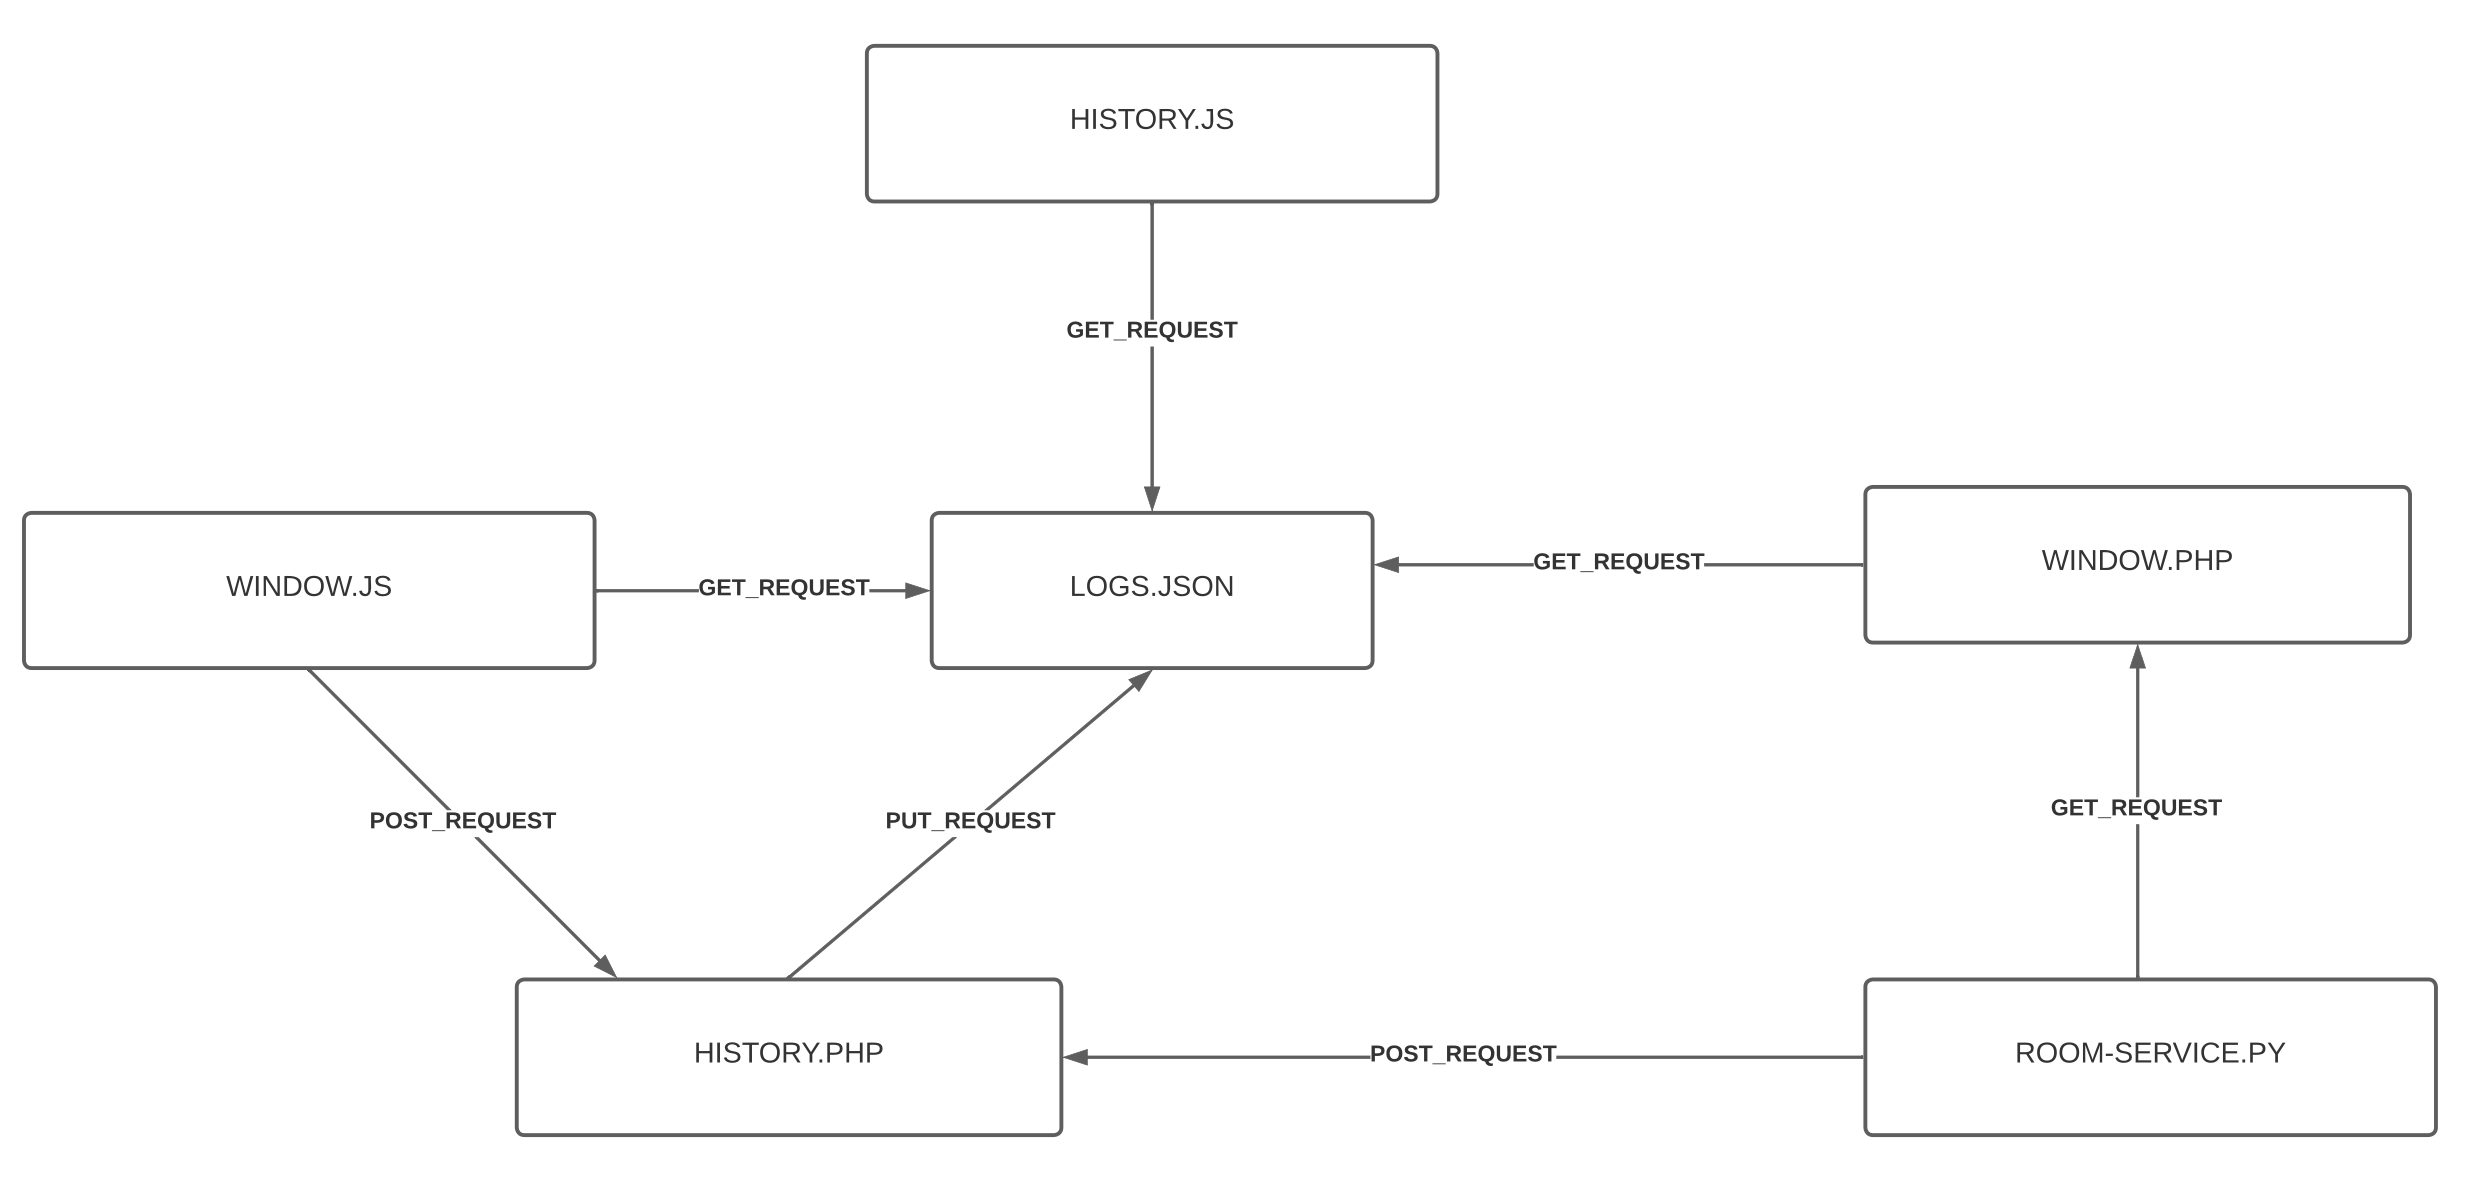
\includegraphics[width=17cm]{dashboard-requests-schema.png}
    \centering
    \caption{Schema funzionamento richieste}
    \centering
\end{figure}

\newpage
% -------------------- Room App --------------------

\section{Room App}



\end{document}
